% TODO: atrophied == degenerated
\documentclass{article}
%\usepackage[top=30pt,left=30pt,right=30pt]{geometry}
\usepackage[german,english]{babel}
\usepackage[utf8]{inputenc}
\usepackage{algpseudocode}
\usepackage{algorithm}
\usepackage{graphicx}
\usepackage{caption}
\usepackage{subcaption}
\usepackage{amsmath}
\usepackage{amssymb}
\usepackage{amsthm}
\usepackage{wasysym}
\usepackage{framed}
\usepackage{xcolor}
\usepackage{makeidx}
\usepackage[pdfborder={0 0 0}]{hyperref}

\usepackage{titlesec}
\titleformat{\paragraph}{\normalfont\itshape}{}{}{}

\newtheorem{theorem}{Theorem}
%\newtheorem{proof}{Proof}
\newtheorem*{hypothesis}{Hypothesis}
\newtheorem*{definition}{Definition}

\algnewcommand{\algorithmicgoto}{\textbf{go to}}%
\algnewcommand{\Goto}[1]{\algorithmicgoto~\ref{#1}}%
\algrenewcommand{\algorithmiccomment}[1]{\hskip2em$\triangleright$ {\footnotesize #1}}

% definitions
\newcommand{\drawing}[1]{%
 \begin{figure}[t]
  \begin{center}
   \includegraphics{#1}
  \end{center}
 \end{figure}
}
\newcommand{\pic}[2]{%
 \begin{figure}[t]
  \begin{center}
   \includegraphics{#1}
   \caption{#2}
  \end{center}
 \end{figure}
}
\newcommand{\cls}[1]{\rm{#1}}
\newcommand{\probl}[1]{\rm{#1}}
\newcommand{\card}[1]{\left|\:\!#1\:\!\right|}
\newcommand{\set}[1]{\left\{#1\right\}}
\newcommand{\given}[1]{\textbf{Given.} #1\par}
\newcommand{\find}[1]{\textbf{Find.} #1\par}
\newcommand{\dateref}[1]{\paragraph{\textit{This lecture took place on #1.}}}
\newcommand{\synonym}[2]{\textbf{Synonym for ``#1''.} #2.\par}
\newcommand{\gath}[2]{$#1$-$#2$-path} % graph theory path
\newcommand{\flow}[2]{$#1$-$#2$-flow}
\newcommand{\exist}{\;\exists\,}
\newcommand{\fall}{\;\forall\,}
\newcommand{\noproof}[1]{A proof for Theorem~\ref{#1} is not provided.}
\makeatletter
\newcommand{\xRightarrow}[2][]{\ext@arrow 0359\Rightarrowfill@{#1}{#2}}
\makeatother

\newcommand\hcancel[2][black]{\setbox0=\hbox{$#2$}%
\rlap{\raisebox{.45\ht0}{\textcolor{#1}{\rule{\wd0}{1pt}}}}#2} 

\DeclareMathOperator{\push}{push}
\DeclareMathOperator{\ex}{ex}
\DeclareMathOperator{\rank}{rank}
\DeclareMathOperator{\detm}{det}
\DeclareMathOperator{\perm}{det}
\DeclareMathOperator{\sign}{sign}
\DeclareMathOperator{\degree}{deg}
\DeclareMathOperator{\prop}{probability}
\DeclareMathOperator{\argmax}{argmax}
\DeclareMathOperator{\argmin}{argmin}
\DeclareMathOperator{\deficiency}{def}

\makeatletter
\providecommand*{\dotcup}{%
  \mathbin{%
    \mathpalette\@dotcup{}%
  }%
}
\newcommand*{\@dotcup}[2]{%
  \ooalign{%
    $\m@th#1\cup$\cr
    \hidewidth$\m@th#1\cdot$\hidewidth
  }%
}
\makeatother


% metadata
\title{
  Combinatorial Optimization 1 \\
  \large{Lecture notes, University of Technology Graz}
}
\date{\today}
\author{Lukas Prokop}

% settings
\parindent0pt
\setlength{\parskip}{0.4\baselineskip}
%\setcounter{tocdepth}{2}

\makeindex

\begin{document}
\begin{theorem}\label{proposition-2.1}
  The MWF problem and MST problem are equivalent.
\end{theorem}
\begin{theorem}\label{satz-2.2}
(Optimality conditions.)
Let $(G, i)$ be an instance of MST and $T$ be a spanning tree in $G$. In this case the following statements are equivalent:
\begin{itemize}
  \item $T$ is optimal
  \item $\fall e = \set{x, y} \in E(G) \setminus E(T)$: no edge of the \gath xy in $T$ has greater weight than $e$
  \item $\fall e \in E(T)$: If $C$ is one of the connected components of $T \setminus \set{e}$, then $e$ is an edge from $\delta(V(c))$ with minimal weight.
  \item $E(T) = \set{e_1, e_2, \ldots, e_{n-1}}$ can be ordered such that $\fall i \in \set{1, 2, \ldots, n-1}$ there is a set $X \subseteq V(G)$ such that $e_i \in \delta(X)$ with minimal weight ad $e_j \neq \delta(X) \fall j \in \set{1, 2, \ldots, i-1}$.
\end{itemize}
\end{theorem}
\begin{theorem}
  $a \Rightarrow b \Rightarrow c \Rightarrow d \Rightarrow a$.
\end{theorem}
\begin{theorem}\label{satz-2.3}
  Krukal's algorithm is correct.
\end{theorem}
\begin{theorem}\label{satz-2.4}
  Let $G$ be a digraph with $n$ vertices. The following 7 statements are equivalent:
\begin{enumerate}
  \item $G$ is an arborescence with root $r$.
  \item $G$ is a branching with $n-1$ edges and $\operatorname{deg}^-(r) = 0$.
  \item $G$ has $n-1$ edges and every vertices is reachable from $r$.
  \item Every vertex is reachable from $r$ and removal of one edge destroys this property.
  \item $G$ satisfies $\delta^+(X) \neq 0 \fall X \subset V(G)$ with $r \in X$. The removal of one arbitrary edge destroys this property.
  \item $\delta^-(r) = 0$ and $\fall v \in V(G) \setminus \set{r} \exists$ one distinct directed $r-v$-path in $G$
  \item $\delta^-(r) = 0$ and $\card{\delta^-(v)} = 1 \fall v \in V(G) \setminus \set{r}$ and $G$ is cycle-free.
\end{enumerate}
\end{theorem}
\begin{theorem}\label{satz-2.5}
  Kruskal's algorithm can be implemented with time complexity $\mathcal{O}(m \log{n})$.
\end{theorem}
\begin{theorem}\label{satz-2.6}
  Prim's algorithm is correct and can be implemented with time complexity of $\mathcal{O}(n^2)$.
  Correctness follows from theorem 2.2.d ($a \Rightarrow b \Rightarrow c \Rightarrow d \Rightarrow a$):
    Spanning tree is optimal $\Leftrightarrow$ order of edges $e_1, \ldots, e_{n-1}$ such that
    $\fall i \in \set{1, 2, \ldots, n-1} \exists x_i \subset V(G)$ with $e_i \in \delta(X_i)$
    is the minimum edge in $\delta(X_i)$ and $e_j \notin \delta(X_i)$ is the cheapest edge of $\delta(X_i)$
    and $e_j \notin \delta(X_i) \fall 1 \leq j \leq i-1$. This is satisfied by construction.
\end{theorem}
\begin{theorem}\label{satz-2.7}
  Is Prim's algorithm implemented with Fibonacci-Heaps we can solve the MST problem in $\mathcal{O}(m + n\log{n})$ time.
  \[
    \mathcal{O}(n^2) \qquad \mathcal{O}(m + n\log{n}) \qquad m = \theta(n^2) \qquad G \text{ is dense}
  \]
\end{theorem}
\begin{theorem}\label{satz-2.8}
  (Arthur Cayley)
  The complete graph $K_n$ has $n^{n-2}$ spanning trees.
\end{theorem}
\begin{theorem}\label{lemma-2.10}
  Let $B_0$ be a subgraph of $G$ with maximum weight and $\deg^-_{B_0}(v) \leq 1 \fall v \in V(G)$.
  Then $\exists$ an optimal branching $B \in G$ with properties $\fall$ cycle $C \in B_0: \card{E(C) \setminus E(B)} = 1$.
\end{theorem}
\begin{theorem}\label{satz-2.11}
Edmonds' Branching Algorithm is correct and computes the branching in $\mathcal{O}(m\cdot n)$.
\end{theorem}
\begin{theorem}\label{proposition-3.1}
Let $G$ be a digraph with conservative weights. $c: E(G) \rightarrow \mathbb{R}$. Let $s, w \in V(G)$ and $k \in \mathbb{N}$. Let $P$ be the shortest among all \gath swes with at most $k$ edges. Let $e = (v, w)$ be the last edge of $P$. Then $P_{[s, w]}$ is the shortest \gath sv with at most $(k-1)$ edges.
\end{theorem}
\begin{theorem}\label{satz-3.2}
  Dijkstra's algorithm is correct and can be implemented in $\mathcal{O}(n^2)$.
\end{theorem}
\begin{theorem}\label{satz-3.3}
  (Fredman and Tarjan, 1987)
  A Fibonacci-Heap implementation of Dijkstra's algorithm runs in $\mathcal{O}(m + n\log{n})$ time.
\end{theorem}
\begin{theorem}\label{satz-3.4}
  The Moore-Bellman-Ford algorithm is correct and has runtime $\mathcal{O}(nm)$.
\end{theorem}
\begin{theorem}\label{satz-3.5}
Let $G$ be a digraph with $c: E(G) \rightarrow \mathbb{R}$. A potential of $(G, c)$ exists iff $c$ is conservative.
\end{theorem}
\begin{theorem}\label{korollar-3.5}
  Let $G = (V, E)$ be a digraph with $c: E(G) \rightarrow \mathbb{R}$. The Moore-Bellman-Ford algorithm can either determine a desired potential or find a negative cycle in $\mathcal{O}(m\cdot n)$ .
\end{theorem}
\begin{theorem}\label{satz-3.6}
  The Floyd-Warshall algorithm works correctly and has a runtime of $\mathcal{O}(n^3)$
\end{theorem}
\begin{theorem}\label{satz-3.10}
  (Karp 1978.)
  Let $G$ be a digraph with $c: E(G) \rightarrow \mathbb{R}$. Let $s \in V(G)$ such that $\fall v \in V(G) \setminus \set{s} \exists$ directed \gath sv in $G$.
  \[
    \fall x \in V(G) \fall K \in \mathbb{Z}_+:
  \] \[
    F_K(x) := \min\set{
      \sum_{i=1}^k c(v_{i-1}, v_i):
        v_0 = s, v_k = x, (v_{i-1}, v_i) \in E(G),
        \fall 1 \leq i \leq k
    }
  \]

  If there is no sequence of edges of length $k$ from $s$ to $x$, then $F_K(x) = \infty$.
  Set $\mu(G, c)$ be the minimal mean edge weight of a cycle in $(G, i)$ and $\mu(G, c) = \infty$ if $G$ is acyclic. Then it holds that
  \[
    \mu(G, c) = \min_{x \in V(G)} \max_{0 \leq k \leq n-1} \frac{F_n(x) - F_k(x)}{n-k}
  \]
\end{theorem}
\begin{theorem}\label{korollar-3.11}
  The minimal mean cycle works correctly and can be implemented with a runtime of $\mathcal{O}(n \cdot\max\set{m,n})$.
\end{theorem}
\begin{theorem}
  \label{proposition-4.1}
  MFP always has an optimal solution. Linear programming always provides an optimal solution and is limited by $\sum_{e \in E(G)} u_e$.
\end{theorem}
\begin{theorem}
  \label{lemma-4.2}
  $\forall A \subsetneqq V(G)$ with $s \in A, t \notin A$ and for every $s$-$t$-flow it holds that:
  \begin{enumerate}
    \item $\operatorname{value}{(f)} = \sum_{e \in \delta^+(A)} f(e) - \sum_{e \in \delta^-(A)} f(e)$
    \item $\operatorname{value}{(f)} \leq \sum_{e \in \delta^+(A)} u_e$
  \end{enumerate}
\end{theorem}
\begin{theorem}\label{lemma-4.3}
  Let $(G, u, s, t)$ be a network and $f$ be a flow. If there is no \gath st in $G_f$,
  then $f$ is optimal. Hence $\operatorname{value}(f)$ is at maximum.
\end{theorem}
\begin{theorem} \label{satz-4.4}
  (\emph{Max flow, min cut problem}, Ford \& Fulkerson, 1956)
  Let $(G, u, s, t)$ be a network than there exists a maximal \flow st $f$
  and a minimal cut ($s$-$t$-cut) $\delta^+(A)$ with $\operatorname{value}(f) = u(\delta^+(A))$.
  Especially the value of a maximal flow and the capacity of a minimal $s$-$t$-cut is equal.
\end{theorem}
\begin{theorem}\label{satz-4.5}
  \textbf{Flow decomposition theorem} (Galler 1956, Ford and Fulkerson 1962)
  Let $(G, u, s, t)$ be a network and $f$ be a \flow st. Then $\exists$ a family
  $\mathcal{P}$ of \gath sts and a family $\mathcal{C}$ of cycles in $G$ and the
  weights in $\mathcal{P} \cup \mathcal{C} \rightarrow \mathbb{R}_+$
  ($P \mapsto w(P), C \mapsto w(C)$) such that
  \begin{align*}
    f(e) = \sum_{P \in \mathcal{P} \cup \mathcal{C}: e \in E(P)} w(P) \fall e \in E(G)
  \end{align*}
  \begin{align*}
    \operatorname{value}(f) = \sum_{p \in \mathcal{P}} w(P)
      \quad\text{and}\quad
      \card{\mathcal{P}} + \card{\mathcal{C}} \leq \card{E(G)}
  \end{align*}
\end{theorem}
\begin{theorem}\label{lemma-4.6}
  Let $f_0, f_1, \ldots, f_k, \ldots$ be a sequence of flows created by the E\&K algorithm, where $f_{i+1} = f_i + P_i$ and $P_i$ is a shortest \gath st in $G_{f_i} \fall i$. Then it holds that
  \begin{itemize}
    \item $\card{E(P_k)} \leq \card{E(P_{k+1})} \fall i$
    \item $\card{E(P_k) + z \leq \card{E(P_r)}}$ for all $k < r$ such that $P_k \cup P_r$ contains at least one pair of edges of opposing direction.
  \end{itemize}
\end{theorem}
\begin{theorem}\label{satz-4.6}
  (Edmonds and Karp, 1972)
  The algorithm of Edmonds and Karp requires at most $\frac{nm}2$ augmented paths (equals to the number of iterations) and determines a maximum flow correctly. The algorithm has a runtime complexity of $\mathcal{O}(m^2 \cdot n)$.
\end{theorem}
\begin{theorem}\label{satz-4.7}
  Dinitz' algorithm finds a maximum flow in $\mathcal{O}(n^2m)$ runtime.
\end{theorem}
\begin{theorem}\label{proposition-4.8}
  The push-relabel algorithm has two invariants:
  \begin{itemize}
    \item $f$ is always an $s$-$t$-preflow
    \item $\psi$ is always a corresponding distance marker
  \end{itemize}
\end{theorem}
\begin{theorem}\label{lemma-4.9}
  Let $f$ be a preflow and $\psi$ be a distance marker in regards of $f$. Then the following statements hold:
  \begin{enumerate}
    \item $s$ is reachable from every active vertex $v$ in $G_f$.
    \item If $v, w \in V(G)$ with $w$ being reachable from $v$ in $G_f$,
          then $\psi(v) \leq \psi(w) + n - 1$
    \item $t$ is not reachable in $G_f$
  \end{enumerate}
\end{theorem}
\begin{theorem}\label{satz-4.10}
  When PR algorithm terminates, $f$ is a maximal \flow st.
\end{theorem}
\begin{theorem}\label{lemma-4.11}
  (number of relabel operations)
  \begin{itemize}
    \item $\fall v \in V(G): \psi(v)$ is increased in every relabel operation by at least one (strong monotonicity, no decrement)
    \item $\psi(v) \leq 2n - 1$ is an invariant $\forall v \in V(G)$
    \item No vertex exists which is relabelled more than $2n - 1$ times. Hence the maximum number of relabel operations is $2n^2 - n$
  \end{itemize}
\end{theorem}
\begin{theorem}\label{lemma-4.12}
  The number of saturating push operations is $2nm$.
\end{theorem}
\begin{theorem}\label{lemma-4.13}
  \emph{Number of non-saturating push operations.}
  The number of non-saturating push operations is $\mathcal{O}(n^2m)$.
\end{theorem}
\begin{theorem}\label{lemma-4.14}
  \emph{Better analysis for number of non-saturating push operations. Cheriyan and Mehlhorn 1999.}
  If the algorithm always select an active vertex with maximum $\psi(v)$, then the push-and-relabel algorithm only requires $8n^2 \sqrt{m}$ non-saturating push operations.
\end{theorem}
\begin{theorem}\label{satz-4.15}
  The push-and-relabel algorithm solves the maximum-flow problem correctly and can be implemented with $\mathcal{O}(n^2 \sqrt{m})$ runtime.
  (with selection of active vertices as in Theorem~\ref{lemma-4.14})
\end{theorem}
\begin{theorem}\label{lemma-4.5}
  For every triple of vertices $i, j, k \in V(G)$ (G is an undirected graph) it holds that
  \[
    \lambda_{i,k} \geq \min{\set{\lambda_{i,j}, \lambda_{j,k}}}
  \]
\end{theorem}
\begin{theorem}\label{lemma-4.16}
  Let $G$ be an undirected graph and $u: E(G) \rightarrow \mathbb{R}_+$.
  Let $s, t \in V(G)$ and $\delta(A)$ a minimal $s$-$t$-cut in $(G', u')$.
  $(G', u')$ results from $(G, u)$ by contraction of $A$ by a single vertex $K$.
  Let $s', t' \in V(G) \setminus A$. Then it holds that
  \[
    \forall \min{\text{s'-t'-cuts}}: \delta(K \cup \set{A}) \text{ is }
      \delta(K \cup A) \text{ a minimal s'-t'-cut in } (G, u)
  \]
\end{theorem}
\begin{theorem}\label{lemma-4.17}
  After every iteration of step 4, the following conditions hold:
  \begin{itemize}
    \item $A \mathop{\dot{\cup}} B = V(G)$
    \item $E(A, B)$ is a minimal $s$-$t$-cut in $(G, u)$
  \end{itemize}
  \[
    A, B \subseteq V(G)  \qquad  E(A, B) := \set{e \in E(G): e = (x, y) \quad x \in A, y \in B}
  \]
\end{theorem}
\begin{theorem}\label{lemma-4.18}
  Invariant of the algorithm:
  \[
    w(e) = u(\delta_G(\bigcup_{z \in C_e} Z)) \fall e \in E(T)
  \]
  where $c_e$ and $V(T) \setminus c_e$ are the two connected components of $T - e$.
  Furthermore it holds that
  \[
    \forall e = \set{P, Q} \in E(T)
      \quad \exists p \in P
      \quad \exists q \in Q \text{ with } \lambda_{p,q} = w(e)
  \]
\end{theorem}
\begin{theorem}\label{satz-4.19}
  The Gomory-Hu algorithm works correctly.
  Every undirected graph contains a Gomory-Hu tree which can be computed in runtime $\mathcal{O}(n^3 \sqrt{m})$.
\end{theorem}
\begin{theorem}\label{proposition-4.20}
  In an undirected graph $G$ with $u: E(G) \rightarrow \mathbb{R}_+$ we can compute a MA-order in $\mathcal{O}(m + n\log{n})$ time.
\end{theorem}
\begin{theorem}\label{lemma-4.21}
  Let $G$ be an undirected graph with $u: E(G) \rightarrow \mathbb{R}_+$ and MA-order $u_1, \ldots, u_n$.
  Then it holds that
  \[
    \lambda_{v_{n-1}, v_n} = \sum_{e \in E(\set{v_n}, \set{v_1, \ldots, v_{n-1}})}
  \]
\end{theorem}
\begin{theorem}\label{satz-4.22}
  A cut of minimal capacity in an undirected graph $G$ with $u: E(G) \rightarrow \mathbb{R}_+$ can be computed with $\mathcal{O}(nm + n^2 \log{m})$ runtime.
\end{theorem}
\begin{theorem}\label{proposition-5.1}
  Let $G$ be a digraph with capacity $u: E(G) \rightarrow \mathbb{R}_+$. Let $f$ and $f'$ be $b$-flows in $G$. Then $g: \overleftrightarrow{E}(G) \rightarrow \mathbb{R}$ with $g(e) = \max\set{0,f'(e) - f(e)}$ and $g(\overleftarrow{e}) = \max\set{0, f(e) - f'(e)} \fall e \in E(G)$ is a \emph{circulation} in $\overleftrightarrow{G} := (V(G), \overleftrightarrow{E}(G))$. Furthermore it holds that $g(e) = 0 \fall e \in \overleftrightarrow E(G) \setminus E(G_f)$ and $c(g) = c(f') - c(f)$.
\end{theorem}
\begin{theorem}\label{proposition-5.2}
  For every circulation $f$ in a digraph $G$ there is a family $\mathcal{C}$ of at most $E(G)$ cycles in $G$ and positive numbers $h(C) \fall c \in \mathcal{C}$ with
  \[
    f(e) = \sum_{c \in \mathcal{C}, e \in E(C)} h(e)
  \]
\end{theorem}
\begin{theorem}\label{satz-5.3}
  (Klein, 1967)
  Let $(G, u, b, c)$ be an instance of MKFP. A $b$-flow $g$ has minimum costs exactly iff there are no $f$-augmented cycles with negative costs in $G_f$.
\end{theorem}
\begin{theorem}
  (Corollary.)
  A $b$-flow has minimum costs iff $(G_f, C_f)$ has a (valid) potential function.
\end{theorem}
  \begin{theorem}
    $x$ \text{ optimal} $\Rightarrow \exists$ optimal solution $(2_e)_{e \in E(G)}, (y_v)_v \in V(G)$
    of DLP with non-satisfied complementary slack.
  \end{theorem}
\begin{theorem}\label{lemma-5.5}
  Let $f_1, f_2, \ldots, f_K$ be a sequence of $b$-flows such that for all $i = 1, 2, \ldots, k-1$:
  $\mu(f_i) < 0$  and $f_{i+1}$ originates from $f_i$ by augmenting $f_i$ along cycle $K_i$ in $G_{f_i}$ ($f_{i+1} = f_i \oplus K_i$).

  For now let $K_i$ be a cycle with minimal average weight in $G_f$. Then the following statements hold:
  \[ \mu(f_i) \leq \mu(f_{i+1}) \fall i \]
  \[ \mu(f_i) \leq \frac{n}{n-2} \mu(f_c) \fall i < l \]
  with property that $K_i \cup K_l$ contains at least one pair of edges of opposing direction.
\end{theorem}
  \begin{theorem}
    \textbf{(Corollary)}
    During the MMCC algorithm $\card{\mu(f)}$ is decremented all $m\cdot n$ iterations by at least factor $\frac12$.
  \end{theorem}
\begin{theorem}\label{proposition-5.6}
  Assume $c: E(G) \rightarrow Q$ (without loss of generality: $c: E(G) \rightarrow \mathbb{Z}$) it holds that:
  after $\mathcal{O}(nm \log_2{n} \card{c_{\text{min}}})$ iterations the MMCC algorithm terminates with
  $c_{\text{min}} = \min\set{\pm c_e | e \in E(G)}$.
\end{theorem}
\begin{theorem}\label{satz-5.7}
  (Tarjan, Goldberg, 1989)
  The MMCC algorithm can be implemented with $\mathcal{O}(m^3 n^2 \log{n})$ runtime.
\end{theorem}
\begin{theorem}\label{satz-5.8}
  Let $(G, u, b, c)$ an instance of MKFP and $f$ be a $b$-flow with minimum costs.
  Let $P$ be a shortest \gath st in regards of $c_f$ in $G_f$ for any $s, t \in V(G_f)$.
  $f'$ results from $f$ by augmentation along $P$ by $\gamma \leq \min\set{u_f(e): e \in E(P)}$,
  hence
  \[
    f'(e) = \left\{\begin{array}{lc}
      f(e) & e \notin E(P), \overleftarrow{e} \notin E(P) \\
      f(e) + \gamma & e \in E(P) \\
      f(e) - \gamma & \overleftarrow{e} \in E(P)
    \end{array}\right\}
  \]

  Then $f'$ is a $b'$-flow with minimum costs where
  \[
    b'(v) = \left\{\begin{array}{lc}
      b(v) & \fall v \notin \set{s,t} \\
      b(v) + \gamma & v = s \\
      b(v) - \gamma & v = t
    \end{array}\right\}
  \]

  \begin{figure}[ht]
   \begin{center}
    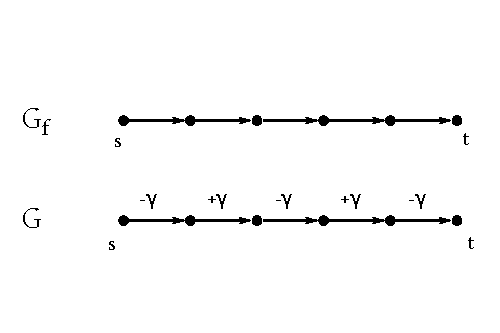
\includegraphics{img/satz_5_8.pdf}
    \caption{Proof of theorem~\ref{satz-5.8}}
   \end{center}
  \end{figure}
\end{theorem}
\begin{theorem}\label{lemma-5.10}
  Let $G$ be a digraph with $u: E(G) \rightarrow \mathbb{R}_+$ and $b: V(G) \rightarrow \mathbb{R}$
  \[ \sum_{v \in V(G)} b(v) = 0 \]
  \begin{equation*}
    \exists \text{ $b$-flow in } G \Leftrightarrow \forall X \subseteq V(G) \text{ it holds that:}
  \end{equation*} \begin{equation*}
    \sum_{e \in \delta^+(X)} u(e) \geq \sum_{v \in V(X)} b(v)
  \end{equation*}
\end{theorem}
\begin{theorem}\label{proposition-5.9}
  If the algorithm terminates with ``there does not exist a $b$-flow in $G$'',
  this statement is correct.
\end{theorem}
\begin{theorem}\label{satz-5.10}
  If $u: E(G) \rightarrow \mathbb{Z}_+, b: V(G) \rightarrow \mathbb{Z}$ and $c$ is conservative,
  the successive shortest path algorithm can be implemented in $\mathcal{O}(nm + B(m + n \log{n}))$.
\end{theorem}
\begin{theorem}
  In every i-th iteration of the algorithm a potential function $\pi$ exists:
  \[
    \pi: V(G) \rightarrow \mathbb{R} \text{ in } G_{f_i}(c_{f_i}(u,v) + \pi(u) - \pi(v) \geq 0)
    \fall e \in E(G_{f_i})
  \]
\end{theorem}
\begin{theorem}\label{satz-5.11}
  (Edmonds and Karp, 1972)
  The capacity scaling algorithm solves the MKFP with integers $b$, infinite capacities and conservative weights correctly. The algorithm can be implemented in $\mathcal{O}(n (m + n \log{n}) \log{b_{\text{max}}})$ runtime where $b_{\text{max}} := \max\set{b(v): v \in V(G)}$.
\end{theorem}
\begin{theorem}\label{satz-5.21}
  (Ford, Fulkerson, 1958)
  The MFoTP can be solved with the same time complexity like MKFP.
\end{theorem}
\begin{theorem}\label{satz-6.1}
  (Berge, 1957)
  Let $M$ be a matching in $(G, E)$. $M$ is maximal if and only if there is no $M$-augmenting path in $G$.
\end{theorem}
\begin{theorem}\label{satz-6.2_}
  Let $G = (v_1 \dotcup v_2, E)$ be a bipartite graph. Then it holds $v(G) = \zeta(G)$.
\end{theorem}
\begin{theorem}\label{satz-6.3}
  (Hall's marriage condition.)
  Let $G$ be a bipartite graph $(A \dotcup B, E)$ then $G$ has a covering matching for $A$ if and only if $\card{\Gamma(X)} \geq \card{X} \fall X \subseteq A$ where $\Gamma(X) = \set{b \in B: \exists a \in X, (a, b) \in E(G)}$.
\end{theorem}
\begin{theorem}\label{heiratssatz}
  (Marriage corollary.)
  Let $G$ be a bipartite graph with $V(e) = A \dotcup B$ and $\card{A} = \card{B}$.
  $G$ has a perfect matching if and only if $\fall X \subseteq A$ with $\card{\Gamma(X)} \geq \card{X}$ holds.
\end{theorem}
\begin{theorem}
  %\textbf{Proposition.}
  Let $G$ be a graph, then
  \[ q_G(X) - \card{X} \equiv \card{V(G)} \mod{2} \fall X \subseteq V(G) \]
\end{theorem}
\begin{theorem}\label{satz-6.6}
  Let $G$ be a graph. $G$ contains a perfect matching if and only if the Tutte condition is satisfied,
  hence $q_G(X) \leq \card{X} \fall X \subseteq V(G)$.
\end{theorem}
\begin{theorem}
  \index{Tutte theorem}
  \index{Theorem by Tutte}
  (Theorem by Tutte.)
  Let $G$ be a graph with a perfect matching
  $\Leftrightarrow$ $q_G(x) \leq \card{X} \fall X \subseteq V(G)$ (tutte condition).

  Less formally:
  A graph $G = (V, E)$ has a perfect matching if and only if every subgraph $G'$
  of any $U \subseteq V(G)$ has at most $\card{U}$ connected components
  with an odd number of vertices.
\end{theorem}
\begin{theorem}\label{proposition-6.7}
  Let $M$ be a matching in $M$ in $G$ and $T$ be an alternating degenerated tree.
  Then $G$ has no perfect matching.
\end{theorem}
\begin{theorem}\label{proposition-6.8}
  Let $C$ be an odd cycle in $G$ and let $G'$ be a graph which results by contraction of $C$.
  Let $M'$ be a matching in $G'$. Then there exists a matching $M$ in $G$ with
  \begin{itemize}
    \item $M \subset M' \cup E(C)$
    \item the number of non-matched vertices of $M$ in $G$ equals the number of non-matched vertices of $M'$ in $G'$
  \end{itemize}
\end{theorem}
\begin{theorem}\label{proposition-6.9}
  Let $G'$ be a graph constructed by iterative contraction of odd cycles as in Edmonds Blossom Algorithm. Let $M'$ be a matching in $G'$ and $T$ be a $M'$-alternating tree in $G$, such that $\fall w \in A(T)$ is $w$ a contracted vertex.

  It follows if $T$ becomes atrophied (no edges left), then $G$ has no perfect matching.
\end{theorem}
\begin{theorem}\label{satz-6.10}
  Edmonds Blossom Algorithm terminates after $\mathcal{O}(n)$ matching augmentations,
  $\mathcal{O}(n^2)$ contractions and $\mathcal{O}(n^2)$ extensions of the tree.
  It decides correct whether a perfect matching exists.
\end{theorem}
\begin{theorem}\label{satz-6.11}
  Edmonds Blossom Algorithm can be implemented with runtime $\mathcal{O}(nm\log{n})$.
\end{theorem}
\begin{theorem}\label{satz-7.2_}
  The assignment problem can be solved with $\mathcal{O}(nm + n^2\log{n})$ runtime.
\end{theorem}
\begin{theorem}\label{satz-7.1}
  (Hoffman \& Kruskal, 1956)
  Let $A \in \mathbb{Z}^{m \times n}$. The following statements are equivalent:
  \begin{enumerate}
    \item $A$ is total unimodular.
    \item Polyeder $P(b) := \set{x \in \mathbb{R}^n: Ax \leq b, x \geq 0}$ is integral $\fall b \in \mathbb{Z}^m$
    \item Every quadratic regular submatrix of $A$ has an integral inverse
  \end{enumerate}
\end{theorem}
\begin{theorem}\label{satz-7.2}
  (Heller \& Tompkins, 1959)
  Let $A \in \set{0, \pm 1}^{m \times n}$ with at most two non-zero eintries per column.
  $A$ is total unimodular if there exists a partition $(R, T)$ of the rows in $A$ $(R \dotcup T = \set{1, 2, \ldots, m}$) such that
  \begin{itemize}
    \item if column $j$ contains two $\pm 1$ entries, then the corresponding rows belong to different parts of the partition.
    \item if column $j$ contains one $+1$ and one $-1$ entry, then the corresponding rows belong to the same part of the partition.
  \end{itemize}
\end{theorem}
\begin{theorem}
  (Corollary by Hoffman and Kruskal)
  Let $A$ be total unimodular with $A \in \set{0, \pm 1}^{m \times n}$.
  \begin{enumerate}
    \item Then it holds that
      \[
        \fall c \in \mathbb{Z}^n, \fall b \in \mathbb{Z}^m:
          \begin{array}{rl}
            P_p &= \set{x \in \mathbb{R}^n: Ax \leq b, x \geq 0} \\
            P_d &= \set{y \in \mathbb{R}^m: A^t y \geq c, y \geq 0}
          \end{array}
      \]
      $P_p$ and $P_d$ are integral.
    \item Polyeder $S = \set{x \in \mathbb{R}^n: \underline{b} \leq Ax \leq \overline{b}, 0 \leq x \leq d}$
      is integral if $\underline{b}, \overline{b} \in \mathbb{Z}^m$ and $d \in \mathbb{Z}_+^n$.
  \end{enumerate}
\end{theorem}
\begin{theorem}
  (Theorem by Birckhoff)
  The permutation matrices correspond to the corners of an assignment polytop and every double-stochastic matrix can be represented as convex combination of permutation matrices.
\end{theorem}
\begin{theorem}
  \label{proposition-8.1}
  The following IDS are matroids
  \begin{enumerate}
    \item $E$ is set of column vectors of a matrix $A$ over an arbitrary field $K$.
      \[
        \mathcal{F} := \set{F \subseteq E: \text{vectors of } F \text{ are linearly independent in } K}
            \qquad \text{``vector matroid''}
      \] \[
        Y = \set{\text{col}_1, \text{col}_2, \ldots \text{col}_k} \fall \in \mathcal{F}
      \] \[
        X = \set{
          \underbrace{\overline{\text{col}_1}, \overline{\text{col}_2}, \ldots, \overline{\text{col}_l}}_{\text{linear indep.}}
        } \in \mathcal{F} \qquad l > k
      \]

      Consider $X \cup Y$: $\rank(X \cup Y) \geq l$ and $\rank(Y) = k < \rank(X \cup Y)$.
      Then it follows that
      \[
        \exists \text{vector } v \in X \cup Y \text{ with } Y \cup \set{u}
        \text{ linearly independent } v \in X \setminus Y
      \]

    \item IDS of exercise $6$. ``\emph{Graphical matroids}''. \index{graphical matroid}
      $X, Y$ forests in $G: \card{X} > \card{Y}$ with (M3) condition. Show that $\exists x \in \mathcal{X}: Y \cup \set{x}$ is forest.

      Assumption: $\fall x \in X: Y \cup \set{x}$ is not a forest $\Leftrightarrow$ $x$ is in a connected component of $Y \fall x \in X$.

      $\Rightarrow$ every connected component of forest $X$ is a subset of a connected component of forest $Y$.


      For any $G = (V, E)$ if $G$ is cycle-free it holds that
      \[ \card{\text{connected components}} = \card{V(G)} - \card{E(G)}  \]
      \begin{align*}
        p &:= \card{\text{connected components of } X} \\
        q &:= \card{\text{connected components of } Y}
      \end{align*}
      \[
        p \geq q
      \] \[
        p = \card{V(G)} - \card{X} \geq \card{V(G)} - \card{Y}
      \]
      As far as $\card{X} \leq \card{Y}$, this is a contradiction.

      \begin{framed}
        \begin{description}
          \item[Tree] number of connected components = $n - (n-1)$. \\
          \item[Forest] number of connected components = $\card{V(G)} - \card{E(G)}$ if $G$ is cycle-free.
        \end{description}
      \end{framed}

    \item ``\emph{Uniform matroid}''. \index{Uniform matroid}
      \[ E = \set{e_1, \ldots, e_n} \quad \mathcal{F} := \set{F \subseteq E: \card{F} \leq k} \]
      with $k \in \mathbb{N}$. $(M3)$ is trivial to show.

    \item $G = (V, E)$ is graph. $S \subseteq V(G)$ stable. $\forall s \in S: k_s \in \mathbb{N}$.
      \[ E = E(G) \quad \mathcal{F} := \set{F \subseteq E(G): \delta_F(s) \leq k_s \fall s \in S} \]
      \[ F = \set{(1, 2), (1, 3), (4, 5), \hcancel{(4, 2)}} \]
      \[ F = \set{(1, 2), (1, 3), (4, 5), (4, 3)} \]

      \begin{figure}[!ht]
        \begin{center}
          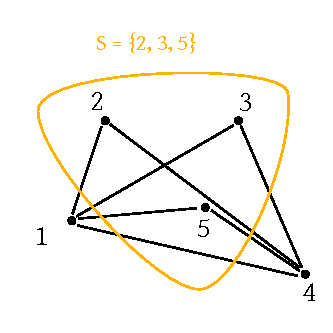
\includegraphics{img/matroid_example_for_4.pdf}
          \caption{Example for Theorem~\ref{proposition-8.1} bullet point 4. $k_2 = 1, k_3 = 2, k_5 = 1$}
          \label{fig:prop81-4-example}
        \end{center}
      \end{figure}

      See figure~\ref{fig:prop81-4-example}.

      (M3) $X, Y \in \mathcal{F}: \card{X} > \card{Y}$.
      \[
        S' = \set{s \in S: \delta_Y(s) = k_s}
      \]
      $\card{X} > \card{Y}$ and $\delta_X(s) \leq k_s \fall s \in S$
      \[
        \xRightarrow{\text{to show}} 
          \exists e \in S \setminus Y
          e \notin \delta(s)
          \fall s \in S'
      \]
      If such an edge exists, we can append it.
      \[
        \Rightarrow Y \cup \set{e} \in \mathcal{F}
      \]

      \begin{figure}[!ht]
        \begin{center}
          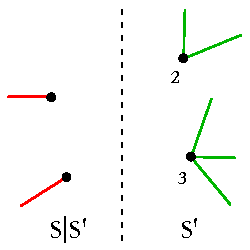
\includegraphics{img/matroid_4_edge.pdf}
          \label{fig:prop81-4-edge}
        \end{center}
      \end{figure}

      Assumption: $\xRightarrow{\text{to show}}$ does \emph{not} hold:
      $\fall e \in X \setminus Y: \exists s \in S': e \in \delta(s)$

      \begin{figure}[!ht]
        \begin{center}
          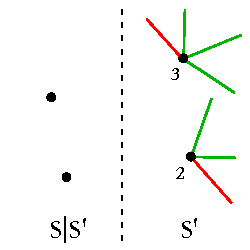
\includegraphics{img/matroid_4_edge2.pdf}
          \label{fig:prop81-4-edge2}
        \end{center}
      \end{figure}

      \[
        \Rightarrow \card{X}
            = \sum_{s \in S'} \delta_X(s) \leq \sum_{s \in S'} ks
            = \sum_{s \in S'} \delta y(s) = \card{Y}
      \] \[
        \card{X} \leq \card{Y}
      \]
      Contradiction to the assumption.

    \item Let $G = (V, E)$ be a digraph. $S \subseteq V(E)$. $k_s \in \mathbb{N} \fall s \in S$. $E = E(G)$.
      \[ \mathcal{F} := \set{F \subseteq E: \delta_k^-(s) \leq k_s} \]
      (M3) analogous as in the previous item \#4, but replace $\delta$ with $\delta^-$.
      Stability is relevant for the rational in item \#4, but because a direction is given here, it is not required.
  \end{enumerate}
\end{theorem}
\begin{theorem}
  \label{satz-6.2}
  Let $(E, \mathcal{F})$ be a IDS. Then the following statements are equivalent:
  \begin{itemize}
    \item[M3:] Let $X, Y \in \mathcal{F}, \card{X} > \card{Y} \Rightarrow \exists x \in X \setminus Y \quad Y \cup \set{x} \in \mathcal{F}$
    \item[M3':] Let $X, Y \in \mathcal{F}, \card{X} = \card{Y} + 1 \Rightarrow \exists x \in X \setminus Y \quad Y \cup \set{x} \in \mathcal{F}$
    \item[M3'':] For every $X \subseteq E$ the bases of $X$ have the same cardinality.
  \end{itemize}
\end{theorem}
\begin{theorem}
  \label{proposition-8.3}
  Let $(E, \mathcal{F})$ be an IDS. Then it holds that $q(E, \mathcal{F}) \leq 1$.
  Furthermore iff $q(E, \mathcal{F}) = 1$ then $(E, \mathcal{F})$ is a matroid.
\end{theorem}
\begin{theorem}
  \label{satz-8.4}
  (Hausmann, Jenkyns, Korte, 1980)
  Let $(E, \mathcal{F})$ be an IDS. If $\fall A \in \mathcal{F} \fall e \in E$,
  $A \cup \set{e}$ contains at most $\rho$ cycles, then it holds that
  \[ q(E, \mathcal{F}) \geq \frac{1}{\rho} \]
\end{theorem}
\begin{theorem}
  \label{satz-8.5}
  (bases)
  Let $E$ be a finite set and $\mathcal{B} \subseteq 2^E$. Family $\mathcal{B}$ is the set of bases of a matroid if and only if the following base axioms are satisfied
  \begin{itemize}
    \item[(B1)] $B \neq \diameter$
    \item[(B2)] $\fall B_1, B_2 \in \mathcal{B}$ and $x \in B_1 \setminus B_2: \exists y \in B_2 \setminus B_1$ with $(B_1 \setminus \set{x}) \cup \set{y} \in \mathcal{B}$.
  \end{itemize}
  If $(B_1)$ satisfies $(B_2)$, then $(E, \mathcal{F})$ is the matroid with base set $\mathcal{B}$ where
  \[ \mathcal{F} = \set{F \subseteq E: \exists B \in \mathcal{B} \text{ with } F \subseteq B} \]
\end{theorem}
\begin{theorem}
  \label{satz-8.6}
  Let $E$ be a finite set and $r: 2^E \rightarrow \mathbb{Z}_+$. Then the following 3 statements are equivalent:
  \begin{itemize}
    \item $r$ is the rank function of a matroid $(E, \mathcal{F})$ (with $\mathcal{F} = \set{F \subseteq E: r(F) = \card{F}})$.
    \item $\fall X, Y \subseteq E$ it holds that
      \begin{itemize}
        \item[(R1)] $r(X) \leq \card{X}$
        \item[(R2)] $X \subseteq Y \Rightarrow r(X) \leq r(Y)$
        \item[(R3)] $r(X \cup Y) + r(X \cap Y) \leq r(X) + r(Y)$ (submodular)
      \end{itemize}
    \item $\fall X \subseteq E$ and $x, y \in E$ it holds that
      \begin{itemize}
        \item[(R1')] $r(\diameter) = 0$
        \item[(R2')] $r(X) \leq r(X \cup \set{y}) \leq r(X) + 1$
        \item[(R3')] $r(X \cup \set{x}) = r(X \cup \set{y}) = r(X) \Rightarrow r(X \cup \set{x, y}) = r(X)$
      \end{itemize}
  \end{itemize}
\end{theorem}
\begin{theorem}
  \label{satz-8.7}
  (Closure)
  Let $E$ be a finite set with $r: 2^E \rightarrow 2^E$.
  $\sigma$ is the closure function of a matroid if $\fall X, Y \subseteq E$ and $\fall x, y \in E$ it holds that
  \begin{itemize}
    \item[(S1)] $X \subseteq \sigma(X)$
    \item[(S2)] $X \subseteq Y \Rightarrow \sigma(X) \subseteq \sigma(Y)$
    \item[(S3)] $\sigma(\sigma(x)) = \sigma(x)$
    \item[(S4)] $[y \notin \sigma(X) \land y \in \sigma(X \cup \set{x})] \Rightarrow x \in \sigma(X \cup \set{y})$
  \end{itemize}
\end{theorem}
\begin{theorem}
  \label{satz-8.8}
  (Cycles)
  Let $E$ be a finite set and $\mathcal{C} \subseteq 2^E$. $\mathcal{C}$ is the set of cycles of an IDS ($E, \mathcal{F}$) with $\mathcal{F} := \set{F \subseteq E: \nexists C \in \mathcal{C} \text{ with } C \subseteq F}$ if and only if the following conditions are satisfied:

  \begin{itemize}
    \item[(C1)] $\diameter \notin \mathcal{C}$
    \item[(C2)] $\fall C_1, C_2 \in \mathcal{C}: C_1 \subseteq C_2 \Rightarrow C_1 = C_2$
  \end{itemize}

  Furthermore for the set $\mathcal{C}$ of cycles of an IDS it holds that:
  \begin{itemize}
    \item[a)] $(E, \mathcal{F})$ is a matroid
    \item[b)] $\fall X \in \mathcal{F} \fall e \in E: X \cup \set{e}$ contains at most one cycle. Denote this number of cycles as $C(X, e)$. If no cycle exists, let $C(X, e) = \diameter$.
  \end{itemize}
  where $a \Leftrightarrow b$.

  Furthermore this statement is equivalent b)
  \begin{itemize}
    \item[(C3)] $\fall C_1, C_2 \in \mathcal{C}$ with $C_1 \neq C_2 \fall e \in C_1 \cap C_2, \exists C_3 \in \mathcal{C}$ with $C_3 \subseteq (C_1 \cup C_2) \setminus \set{e}$
    \item[(C4)] $\fall C_1, C_2 \in \mathcal{C}, \fall e \in C_1 \cap C_2, \fall f \in C_1 \setminus C_2$ exists $C_3 \in \mathcal{C}$ with $f \in C_3 \subseteq (C_1 \cup C_2) \setminus \set{e}$.
  \end{itemize}
\end{theorem}
\begin{theorem}
  \label{proposition-8.9}
  It holds that $(E, \mathcal{F}^{**}) = (E, \mathcal{F})$
\end{theorem}
\begin{theorem}
  \label{corollary-8.10}
  \label{satz-8.10}
  $B^*$ base of $(E, \mathcal{F}^*) \Leftrightarrow \exists$ base $B$ of $(E, \mathcal{F})$ with $B^* = B^C$ and $(E, \mathcal{F}^*)$ its dual. Let $r$ and $r^*$ be the corresponding rank functions.
  Then it holds that
  \begin{itemize}
    \item[a)] $(E, \mathcal{F})$ is a matroid $\Leftrightarrow$ $(E, \mathcal{F}^*)$ is matroid
    \item[b)] If $(E, \mathcal{F})$ is a matroid, then it holds that $r^*(F) = \card{F} + r(E \setminus F) - r(E) \fall F \subseteq E$
  \end{itemize}
\end{theorem}
\begin{theorem}
  \label{satz-8.11}
  Let $G$ be a connected planar graph with an arbitrary planar embedding.
  Let $G^*$ be the planar duality of $G$. Let $M(G)$ be the graphical matroid of $G$.
  It holds that
    \[ M^*(G) = (M(G))^* = M(G^*) \]

  Furthermore $G$ is planar if and only if $(M(G))^*$ is graphical;
  hence if a graph $G'$ with $M(G') = (M(G))^*$ exists.

  If $G$ is planar, then $G'$ is isomorphic to a planar embedding of $G^*$.
\end{theorem}
\begin{theorem}
  \label{satz-8.12}
  (Jenkyns, Korte, Hausmann, 1978)
  Let $(E, \mathcal{F})$ be an IDS and $c: E \rightarrow \mathbb{R}_+$. Denote $G(E, \mathcal{F}, c)$ as the costs of a solution determined by the BEST-IN-GREEDY algorithm. Denote $\operatorname{OPT}(E, \mathcal{F}, c)$ as the costs of an optimal solution (both for the maximization problem the GREEDY-IN algorithm is tackling).

  Then it holds that
  \[
      q(E, \mathcal{F})
        \leq \frac{G(E, \mathcal{F}, c)}{\operatorname{OPT}(E, \mathcal{F}, c)}
        \underbrace{\leq}_{\text{\tiny{trivial}}} 1
        \fall c: E \rightarrow \mathbb{R}_+
  \]
\end{theorem}
\begin{theorem}
  \label{satz-8.13}
  (Edmonds, Rado, 1971)
  An IDS $(E, \mathcal{F})$ is a matroix if and only if the BEST-IN-GREEDY algorithm provides an optimal solution for the maximization problem $\fall c: E \rightarrow{R}_+$.
\end{theorem}
\begin{theorem}
  \label{satz-8.14}
  (Edmonds 1971, polyedric representation)
  Let $(E, \mathcal{F})$ be a matroid and $r: E \rightarrow \mathbb{Z}_+$ be a rank function.
  Then the matroid polytop $P(E, \mathcal{F})$ (convex hull of incidence vectors of all independent sets) is given by:
  \[ P(E, \mathcal{F}) = \set{x \in \mathbb{R}^{\card{E}}: x \geq 0, \sum_{e \in A} x_e \leq r(A) \fall A \subseteq E} \]
  \[
    F \in \mathcal{F}  \qquad
    \underbrace{x^F(e)}_{\text{incidence vectors}} = \begin{cases} 1 & e \in F \\ 0 & \text{else} \end{cases} \qquad
    \sum_{e \in A} x^F_e = \card{A \cap F} \leq r(A)
  \]
  We conclude: $x^F \in P(E, \mathcal{F}) \fall F \in \mathcal{F}$.
\end{theorem}
\end{document}
